\documentclass[review]{cmpreport}
\usepackage{natbib}
\usepackage{graphicx}
\graphicspath{ {./} }

\title{Third Year Project: Literature Review}
\author{Matthew Taylor}
\registration{100151729}
\supervisor{Dr Rudy Lapeer}
\ccode{CMP-6013Y}

\begin{document}

\maketitle

\begin{section}{Introduction}

\subsection{Aim of the project}
The project aims to implement a first person shooter game which uses procedural generation to provide a novel and interesting gaming experience. There are many ways procedural content generation (PCG) can be applied to games, so this literature review will explore the broad themes of the field to find specific areas to focus on.

\subsection{Areas of knowledge required}
PCG techniques have been developed and used in video games since the 1970s. I will need to gain a strong understanding of this field in order to find interesting areas to focus on.\par
In order to implement the concepts and techniques I will focus on, I will need to learn how to use the Unity platform.

\subsection{Report structure}
The report will provide a summary of the PCG field, identifying key themes and the current state of the field, including interesting "unsolved problems" or under-explored areas. \par
I will then focus on a few promising areas to explore the literature in detail, with a view to informing my project's aim and objectives. \par
This report will critically analyse sources as they are referenced. This will inform my conclusions and amendments to my project's aim and objectives, which I will present at the end of the report.

\end{section}

\begin{section}{Overview of Procedural Content Generation}
\subsection{Types of Procedural Content Generation}
There are two main types of procedural content generation, which use similar methods but achieve different goals. They are \textbf{endless content generation} and \textbf{efficient content storage}.

\subsubsection{Efficient content storage}
Prevalent in the early days of PCG, efficient content storage exploits procedural content generation to create large amounts of data without needing to store it - it can simply be re-generated using a deterministic algorithm every time it is required. An example of this is the 1984 game \textit{Elite}, as documented in \citet{spufford_2003}. Here, the game developers discuss using a pseudorandom number generator with pre-defined seeds to generate large amounts of content, without needing to store any of the content itself. \par
A similar technique is adopted for image generation, as per \cite{Perlin:1985:IS:325165.325247}. Perlin describes using well-defined stochasic functions that can be parametised to produce realistic textures procedurally. This means that textures can be generated when required or when a program is initialised, rather than needing to store them. \par
A lot has changed in computers since the 80s - memory and storage constraints are now much less of an issue, so using PCG to efficiently store large amounts of content has been used less.

\subsubsection{Endless content generation}
As storage constraints have been eclipsed by the rapid development of technology, the generation of content has become more of a concern. Increasing sophistication of games and the expectations of players mean content creation is more time-consuming and costly. This has resulted in an increase in the use of PCG to generate content. \par
This has become a wide field, resulting in the creation of a taxonomy of PCG in \cite{Hendrikx:2013:PCG:2422956.2422957}. It describes six layers of PCG in games:
\begin{enumerate}
    \item Game bits (eg. textures, buildings)
    \item Game space (eg. maps, lakes)
    \item Game systems (eg. roads)
    \item Game scenarios (eg. puzzles, stories)
    \item Game design (eg. rules)
    \item Derived content (eg. leaderboards)
\end{enumerate}

This paper is relatively recent (2013) which makes the summary it provides still accurate to this day. It is cited (36 times on acm.org) by others in the industry. I have done some comparison against http://pcg.wikidot.com/ which maintains a list of games using PCG, which confirms there have been no large advances or practical examples of PCG in games since this was published. This gives me confidence that the taxonomy and techniques discussed are still accurate and relevant today. \par 

\subsection{Areas of PCG to focus on}
In chapter 6 of \cite{Hendrikx:2013:PCG:2422956.2422957}, the paper discusses "recommendations for future research". One of the recommendations details the generation of realistic indoor game spaces. It is also clear from the literature overview that many of the applications of PCG happen before game play begins, so I will be interested to explore the applications of real-time PCG. \par
In the following section, I will narrow my focus to the area of generating indoor spaces, in terms of both layouts and decoration, especially in real-time.

\end{section}

\begin{section}{Procedural generation of indoor spaces}

\subsection{Room generation}
\subsubsection{Agent based approach to decoration}
\cite{doi:10.1111/j.1467-8659.2009.01351.x} describe an agent based approach to decoration, which generates the furniture placement in a room. Agents are assigned to particular objects and, when entering a search state, seek positions that meet particular constraints and goals. It is designed to be deterministic (using PRNGs) and to generate rooms at speed (to avoid storing lots of geometry), when required. These are interesting properties that I would like to explore
further. The authors acknowledge that high-level control and sophistication of the generated layouts are lacking, so these are areas I could look to build on. \par
This paper is now relatively old (2009) and not particularly well cited (22 citations
on Wiley Online Library). It uses relevant techniques (agent based search) but uses
out-dated technology (VRML). The ideas in the paper are interesting and described in
considerable detail, so it is still a useful paper to consider. 

\subsubsection{Computerised clutter}
\cite{taylor-parberry} discuss "computerised clutter" and the challenges involved in making a procedurally generated room look realistic. They list five properties that are desirable in a room generator: novelty, structure, interest, speed and controllability. The paper describes in detail how to procedurally generate "clutter" in a room which does not look computer generated, by using the concept of "anchor points". These points are adjusted with gaussian noise to provide natural looking variation around points and patterns that can be designer-adjusted, making them look human-constructed when in reality they are generated by computers.\par
This paper is very specific although not well cited (1 citation on researchgate.net). It is also not very recent, published in 2010. These facts mean I am not going to read too much into the paper, especially as they primarily present only one technique of generating "computerised clutter". However, their subjective summary of what makes procedural generation of clutter in a room look convincing is useful and compelling enough that I have included it. I will incorporate some of these techniques into the decoration of my room generator.

\subsubsection{Combining human and procedural content generation}
Discussed in the papers above is the idea of content "looking" procedurally generated. Indeed, in the most recent prominent example of a game making extensive use of PCG - No Man's Sky (2016) - is criticised in many reviews, with \cite{welsh_2016} as an example, for being vast but samey. To quote the review: "Some disappointment is inevitable once you've visited a handful of planets and started to see the limits of the algorithm. The parameters of weirdness in No Man's Sky have been quite strictly defined, and it gets repetitive." \par
Rogue-like games tend to suffer less from this phenomenon. A recent example that has been explored in detail is the game Spelunky. As detailed in \cite{gct-spelunky}, Spelunky uses a simple path-finding algorithm, a tile-based approach to generating levels and - crucially - combines human crafted tiles with scope for procedural generation within those tiles. \par
This generates detailed, interesting levels that feel unique, interesting and always have a route from beginning to end. The combination of taking human-designed tiles or areas and integrating procedural elements within them, to provide environments that feel created but are actually generated is intriguing and something I would like to explore further with the project.

\section{Level generation}
\cite{Hendrikx:2013:PCG:2422956.2422957} in Chapter 3 discuss common methods of PCG. In relation to how indoor spaces are generated, they discuss how common methods are Pseudo-random Number Generators (PRNG) and Generative Grammars (GG). \par
These methods are well suited to producing feasible indoor spaces required in games. Although \cite{Hendrikx:2013:PCG:2422956.2422957} detail other techniques, like genetic algorithms and fractal spatial generation, these are less common in games. I suspect this is because the output of layouts they produce, despite being procedurally generated, will either follow a discernable pattern (in the case of fractal algorithms) or will be "too random" (in the case of genetic algorithms) to appeal to human players. My aim is to create a procedural generator that feels realistic in order to be compelling and interesting to the player, so I feel these approaches may not be suitable.

\subsection{Generative grammars}
\cite{Dormans:2010:ALD:1814256.1814257} discusses using generative grammars to create complex, coherent, branching mission and level structures. As the article details, these generate levels more appropriate for action adventure games (as compared to levels generated by roguelikes for roleplaying games) where a pattern and structure to the level is important. The article also details the difference between mission and space. \par
The paper is reasonably well cited (22 citations on acm.org) and was published in 2010. The techniques it describes are certainly not dated and could concievably be used to generate content in games today. \par  
The ideas presented are intriguing, as they specifically reference the type of game I aim to create - a 3D action-adventure style game. The use of GGs will enable sequences of rooms to be generated in which the order matters (for instance, in a maze, a beginning must be connected to a goal position). In this way, it will also be possible to procedurally generate unpredictable layouts that are nevertheless perfectly valid, in an efficient manner.

\subsection{Graph based approaches}
\cite{van2013designing} extends the approach of using generative grammars. They recognise that previous work, especially \cite{sbpcg}, does not focus much on gameplay-based control over the procedural generation. They seek to demonstrate that by using grammars to define constraints, then using graphs to generate constrained content allows a designer to have a hand on the content generated. This is especially useful in the context of games, because it allows generated content to be directed towards something. When things like "realism" and "not looking too computer generated" are considered, this is an interesting concept. \par
Another interesting point they raise is methods of testing the generated content. They use histograms to measure complexity and "danger", which allows them to adjust the constraints to achieve the desired results. They also use histograms to measure the generation speed, which is something I will be focussing on. This is a useful technique and something I will aim to emulate against my own ideas. \par
This paper is more recent than some of the others I have reviewed and cites some of the earlier papers. They specifically address some shortcomings in those papers. This gives me confidence in the areas of the other papers that did not identify as being weak, while also providing useful insight into more modern techniques in PCG. 

\end{section}




\begin{section}{Conclusion}
Through my search of the literature, it is apparent that much of the research and commercial interest in PCG has been for pre-generating content. That is, PCG is used to generate things generally ahead of time and very little in real time. I am interesting in exploring the real-time aspects of PCG, specifically in relation to level layouts of indoor spaces. \par 
This connects with \cite{Hendrikx:2013:PCG:2422956.2422957} that indoor space generation could be explored further, as well as the view in \cite{shaker2016procedural} that PCG could be used as a more "central" element to a game, rather than just a method to generate content. I will make my project aim to explore the idea of real-time layout generation as a fundamental part of the gameplay - something that the game could not exist without. \par
I will explore the following aspects of procedurally generating (and re-generating) level layouts at runtime:
\begin{itemize}
    \item Performance of the game
    \item Fidelity of generated rooms (eg. level of detail that can be generated)
    \item AI pathfinding in shifting layouts
    \item Maintaining valid level states (eg. a game that can always be completed, no matter how much the layout changes)
    \item Making a fun game
\end{itemize}

\subsection{Changes to aims and objectives}
I will change the focus of my project to look more closely at PCG. While I will maintain the initial aim of a game that changes the level layout while it is being played, I will explore this is considerably more detail, especially around the points detailed above. \par 
I will shift focus from AI to PCG of both level layouts and the layout of furniture and decoration in the rooms generated. These are two fields which I believe could be explored in more depth. This is especially true in a run-time context, as very little literature has explored this.

\subsection{Revised gantt chart}
\begin{center}
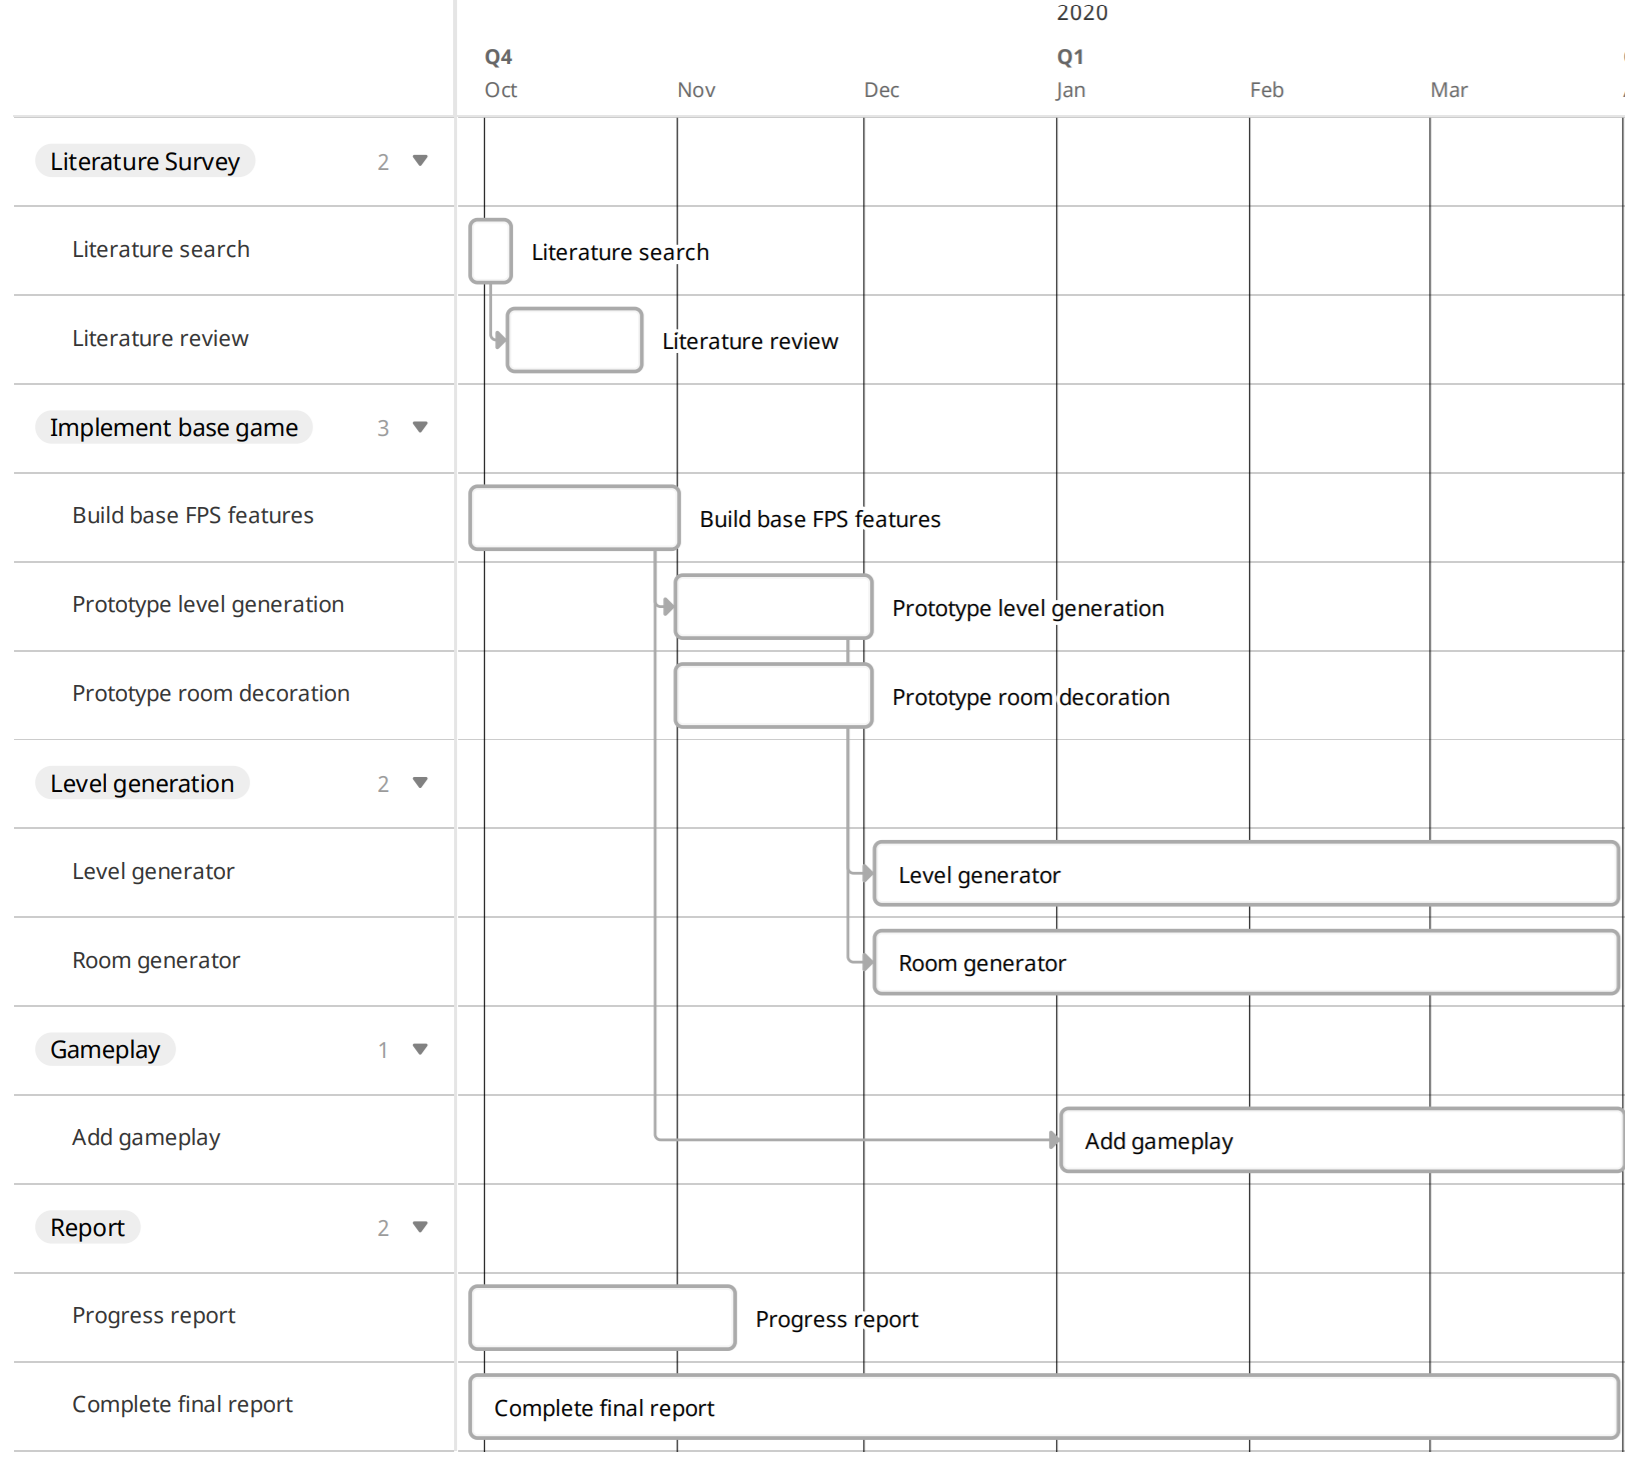
\includegraphics[width=\textwidth,height=\textheight,keepaspectratio]{gantt.PNG}
\end{center}

\subsection{Changes to development approach}
I will also adapt my development approach to more closely align with Agile principles. My timeline will be planned according to the Gantt chart above, but I will run in two week sprints. \par
I will use the sprint review/retrospective time to check my progress against the expected timescales, as well as making notes about performance. Where possible, I will also aim to get user feedback on the general appearance of the generated levels and rooms, in order to gain some insight into their quality.

\end{section}


\bibliography{sources}

\end{document}
